\newpage
\section{Elektrischer Aufbau und Signalverarbeitung}
\label{sec:Elektrischer Aufbau}
Im Zuge der Arbeit wird die Kälteanlage, die zuvor nur manuell betrieben werden konnte, vollständig in eine Struktur einer SPS umgebaut. Zu berücksichtigen ist dabei die Hardware-Schaltschrank-Architektur des manuellen Betriebes. Für den manuellen Betrieb besaß die Kälteanlage zwei Schaltschränke zur Versorgung der Komponenten mit der Hilfsenergie sowie zur Ansteuerung der Magnetventile und des Vierwegeventils.

Um den Umbau auf eine SPS vollziehen zu können, ist es nötig, das elektrische Konzept für den manuellen Betrieb nachzuvollziehen, um  gleiche Funktionalität und Sicherheit der Kälteanlage im SPS-Betrieb gewährleisten zu können. Ein großer Anteil der Komponenten des manuellen Betriebes werden in das neue elektrische Konzept der SPS eingebunden. Nach dem Umbau ist die Kälteanlage ausschließlich über die SPS bedienbar sein.

Das elektrische Konzept sieht eine zentralisierte elektrische Installation vor. Die Verwendung eines Buskopplersystem nicht ist erforderlich. Ein Buskopplersystem wird oft bei zu langen Wegen von analogen Signalen eingesetzt. Analoge Signale können bei zu langer Verkabelung durch elektromagnetische Störquellen verfälscht werden. Messdaten oder auch Stellsignale werden so verfälscht und fehlerhaft. Ein Buskoppler sammelt die Signale und schickt diese dann mittels Ethernet oder EtherCAT zur SPS weiter. 
Bei der Kälteanlage werden die meisten Signale nur über wenige Meter zu den benachbarten Schaltschränken gesendet. Hierbei ist mit keinen Störungen durch elektromagnetische Interferenzen zu rechnen.
 
Folgende Komponenten der Kälteanlage werden elektrisch an die SPS angeschlossen: 
\begin{itemize}
\item	Kompressor-Frequenzregelung geregelt mit einem analogem Ausgangssignal 4\dots 20 mA
\item	Verflüssigungsregelung geregelt mit einem analogem Ausgangssignal  0\dots 20 mA
\item	Elektrische Heizungselemente gesteuert mit einem analogem Ausgangssignal mit 0\dots 10 V
\item	Schaltschütze mit digitalem Ausgangssignal 0/24 V DC für Magnetventile, Vierwegeventil, Spannungsfreigabe für Verdampfer-Ventilatoren
\item 	Modbus RTU über COM-Schnittstelle und RS485-Busklemme
\item 	Waagen-Auslesung über RS232-Schnittstelle
\item 	Pt100- Temperatursensoren
\end{itemize}
 
 
\subsection*{CPU-Grundmodul CX9020 und Busklemmen} 
 
Die SPS besteht aus dem CPU-Grundmodul CX9020 sowie Busklemmen der Fa. Beckhoff. Die Busklemmen sind vom Typ E-Bus, die das firmeneigene Protokoll EtherCAT (Ethernet for Control Automation Technology) unterstützen.  Das EtherCAT verfügt neben ihrer Echtzeitfähigkeit (1.000 verteilte I/Os in 30 $\mu s$\citep{Beckhoff2016}) auch über die Fähigkeit zur Einbindung von  Standardethernet Komponenten und flexiblen Typologien. Bei einem E-Bus (ELxxxx)wird das Prozessabbild mittels des EtherCAT
Protokolls, das vom Standard-Ethernet-Protokoll abgeleitet ist, bis an die jeweilige Busklemme übermittelt. Die Busklemme kann dann ihren Wert lesen bzw. schreiben. Dieses Verfahren erlaubt eine äußerst geringe Zykluszeit. Abbildung \ref{fig:Beckhoffklemmen} zeigt exemplarisch das Grundmodul CX9020 und eine PT100-Temperatur-Busklemme. Der CX9020 verfügt über einen 1-GHz-CPU und läuft mit dem Betriebssystem Windows CE. Es wird auf einer Hutschiene montiert und erkennt angeschlossene Busklemmen automatisch. 

\begin{figure}[htb]
\centering
\subfigure[Ethernet-Steuerungs-CPU CX9020]
{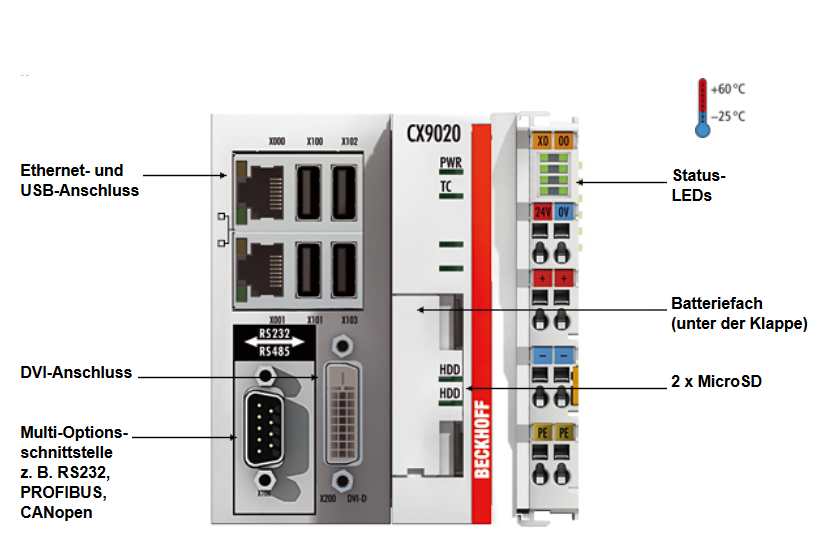
\includegraphics[width=0.52\textwidth]
{Pictures/CX9020.png}}
\subfigure[EL3202: 2-Kanal-Eingangsklemmen für PT100-Temperatursensoren]{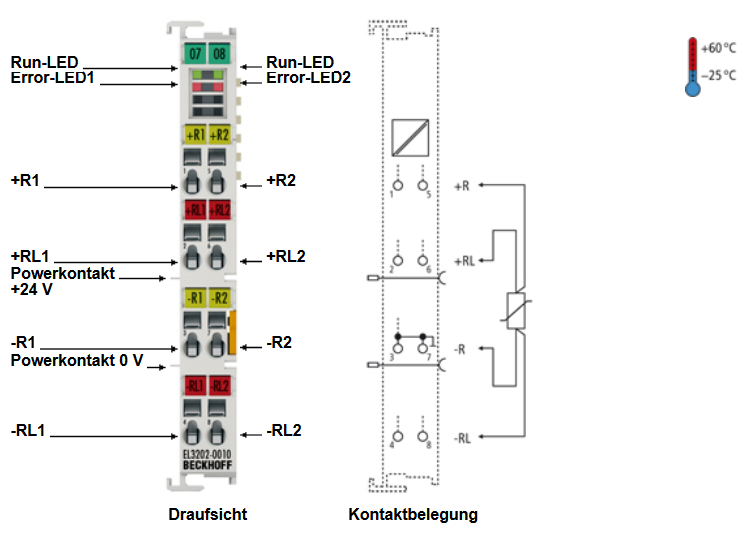
\includegraphics[width=0.42\textwidth]
{Pictures/EL3202.png}}
\caption{SPS-CPU und E-Busklemme der Fa. Beckhoff}
\label{fig:Beckhoffklemmen}
\end{figure}

In Tabelle \ref{tab:Klemmenübersicht} sind alle verwendeten Klemmen mit Kanalanzahl, Signalart und der eingesetzten Anzahl aufgelistet. 

Der CX9020 verfügt über zwei RJ45 Anschlüsse für LAN-Schnittstellen. Hier können weitere Buskoppler oder ein PC angeschlossen werden. Buskoppler kommunizieren über EtherCAT  und der PC über TCP/IP mit dem Gerät. Eine der zwei Schnittstellen dient zur Kommunikation mit dem Host-PC. Vier USB-Schnittstellen dienen für einen Anschluss von beispielsweise einer Maus, Tastatur  oder eines Speichermediums. 

\begin{table}[htb]
\centering
\caption{Busklemmen-Übersicht}\vspace{6pt}
\begin{tabular}{p{2cm}p{3.6cm}p{1.4cm}p{2.8cm}p{3.2cm}ccccc}
\hline 
\rule[-1ex]{0pt}{2.5ex} \textbf{Klemmennummer} & \textbf{Typ} & \textbf{Anzahl Kanäle} & \textbf{Signal} & \textbf{Eingesetze Anzahl} \\ 
\hline 
\hline 
\rule[-1ex]{0pt}{2.5ex} EL 4024 & Analog Ausgang & 4 & 4\dots 20 mA & 1 \\ 
\hline 
\rule[-1ex]{0pt}{2.5ex} EL 4008 & Analog Ausgang & 8 & 0\dots 10 V DC & 1 \\ 
\hline 
\rule[-1ex]{0pt}{2.5ex} EL 3202 & Analog Eingang & 2 & Temperatur & 6 \\ 
\hline 
\rule[-1ex]{0pt}{2.5ex} EL 3054 & Analog Eingang & 4 & 4\dots 20 mA & 1 \\ 
\hline 
\rule[-1ex]{0pt}{2.5ex} EL 2809 & Digital Ausgang & 16 & 24 V DC  & 1 \\ 
\hline 
\rule[-1ex]{0pt}{2.5ex} EL 6021 & Serielle Schnittstelle & 1 &  RS422/RS485 & 1 \\ 
\hline 
\rule[-1ex]{0pt}{2.5ex} EL 9410 & E-Bus Auffrischung & 0 & - & 1 \\ 
\hline 
\rule[-1ex]{0pt}{2.5ex} EL 6002 & Serielle Schnittstellen & 2 & RS232 & 3 \\ 
\hline 
\rule[-1ex]{0pt}{2.5ex} EL 9011 & Endklemme & 0 & - & 1 \\ 
\hline 
\hline 
\end{tabular} 
\label{tab:Klemmenübersicht}
\end{table}



Der CX9020 wird über einen Trafo von der Fa. Siemens mit 24-V-DC versorgt. Über die Kanäle 24-V und 0-V wird der Buskoppler EK 1200 mit Spannung gespeist. Der EK 1200 kommuniziert per E-Bus mit den angeschlossenen Klemmen und versorgt diese über die Powerkontakte mit Spannung.  Der Buskoppler ist in den den CX9020 integriert. Die EK 1200 stellt eine Stromversorgung von \mbox{1860 mA} zur Verfügung.  Jede Klemme hat einen Stromverbrauch im Bereich von 50-190 mA. Eine Unterschreitung der 0 mA Grenze ist möglich, kann laut Hersteller jedoch zu Kommunikationsproblemen führen und ist zu vermeiden. Deshalb wird eine E-Bus-Auffrischungsklemme EL 9410 zur Einspeisung weiterer 1860 mA in den E-Bus integriert. 

Jede Klemme verfügt je nach Ausführung über verschiedene Diagnose-LEDs, die Auskunft über korrekten Anschluss, Betriebsstatus oder eventuelle Fehler geben. Die Kommunikation zu den Busklemmen erfolgt über die Kontakte an der Seite (E-Bus). Abbildung \ref{fig:Beckhoffklemmen} zeigt den CX9020 und eine EL 3202 für zwei PT100-Temperaturelemente. 

Der Beckhoff-Schaltschrank wird über eine separate Spannungsquelle, getrennt von anderen elektrischen Komponenten,  versorgt. Dies erlaubt einen Betrieb der SPS, z. B. fürs Programmieren oder Testen, unabhängig von den anderen Schaltschränken. Für die genaue elektrische Installation wird an dieser Stelle an die Handbücher der jeweiligen Komponenten verwiesen. \citep{MicroNovaAG2011} \citep{KMGH2013} \citep{KERN2006} \citep{KELLER2015} \citep{CAREL2015}

\begin{figure}[htb]
\centering		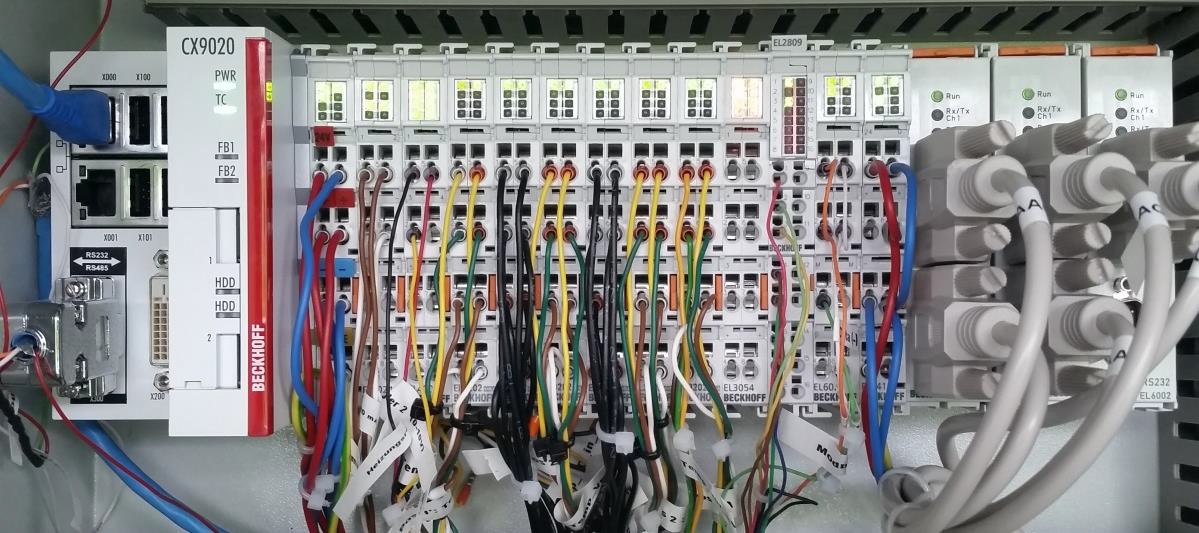
\includegraphics[width=0.90\textwidth]{Pictures/Versuchsaufbau/SPS_BILD.png}
\caption{Verkabelung von CX9020 und Busklemmen}
\label{fig:}
\end{figure}

\newpage
\subsection{RS232-Kommunikation zwischen SPS und KERN-Waage}
\label{subsec:RS232-Verbindung}


%\begin{figure}[htb]
%\centering
%\subfigure[Waage mit separatem Display vom Typ \textit{PCD 10K0.1} der Fa. %\textsc{Kern und Sohn Gmbh} \citep{KERN2006}]%
%{\includegraphics[width=0.4\textwidth]
%{Pictures/Waage.png}}
%\hspace{2cm}
%\subfigure[RS232-Spannungspotentiale von einem nominellen Sender und der EL %6002-Busklemme \citep{Beckhoff2015}]{\includegraphics[width=0.3\textwidth]
%{Pictures/RS232_spannungspotential.png}}
%\caption{Waage und RS232-Kommunikationspotentiale}
%\label{fig:Waage}
%\end{figure}


Das Wägesystem verfügt zurzeit über 5 Waagen, die kontinuierlich von der SPS ausgelesen werden sollen. Jede Waage besteht aus zwei miteinander verbunden Teilen: die Wägeeinheit und das Display mit der RS232-Schnittstelle. Das Datenverbindungskabel zwischen Waage und Display wurde verlängert, sodass sich die Displays in der Nähe des SPS-Schaltkrankes befinden. Der Hersteller empfiehlt die Länge von 2 m für die RS232-Verbindung nicht zu überschreiten.  
Über die Datenschnittstelle kann die Waage Befehle empfangen und Messdaten bzw. Fehlermeldungen senden. 

Eine RS232-Kommunikation arbeitet \textit{bitseriell} und diesem Fall mit einem 8-bit ASCII-Code. RS232 ist eine Spannungsschnittstelle. Binäre Zustände werden durch unterschiedliche Spannungspegel realisiert und versendet. \citep{Schleicher2005}

Hierfür wird ein serielles D-Sub-Kabel benutzt, das an einem Ende einen männlichen D-Sub-Stecker für die EL 6002-Busklemme hat und einen weiblichen D-Sub-Stecker für die Waagen-Schnittstelle. Abbildung \ref{fig:RS232} zeigt die Verkabelung für die RS232-Kommunikation. 

Die Waagen sind in der Klimakammer aufgestellt und ihre Sendeeigenschaften  werden in den Einstellungen auf \textit{AU PC} gestellt. Die Waagen senden dadurch kontinuierlich ihre aktuellen Messdaten an die Klemme, ohne Aufforderung der SPS. Auch wenn die Werte instabil sind, werden sie gesendet. Die Auslesung der gesendet Daten bzw. des Prozessbildes erfolgt dann über Funktionsbausteine und Programme auf der SPS, siehe Abschnitt \ref{sec:Informationstechnischer Aufbau}.


\begin{figure}[htb]
\centering		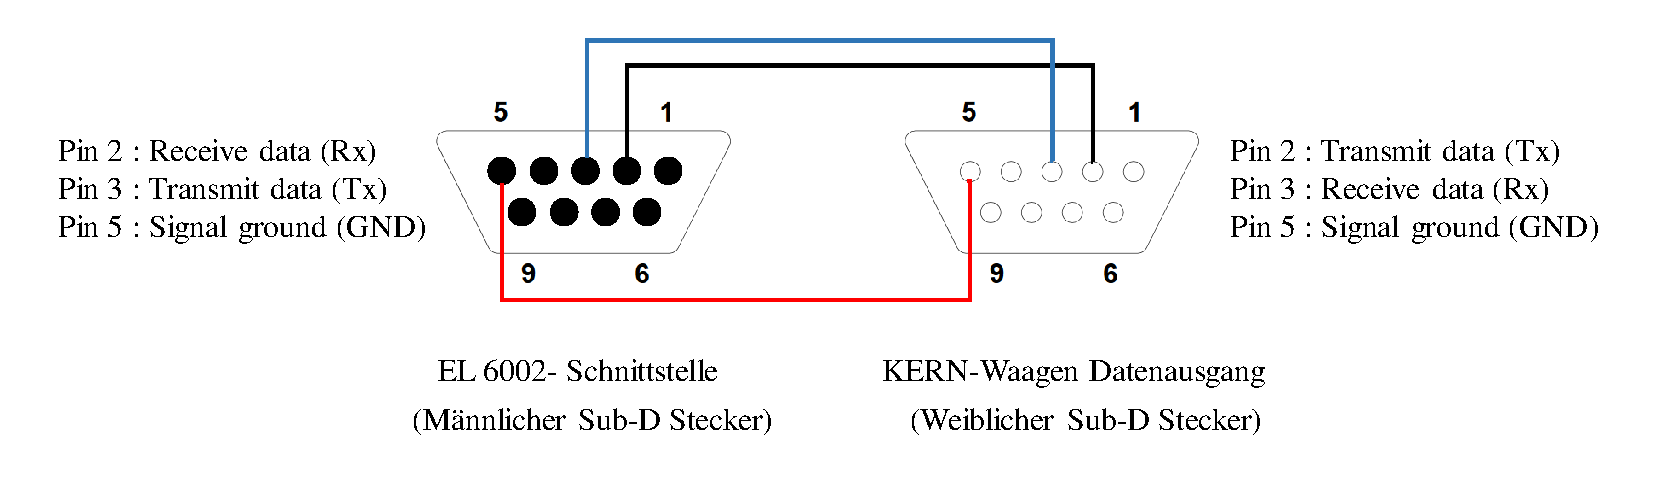
\includegraphics[width=1.05\textwidth]{Pictures/RS232_Verkabelung.pdf}
\caption{Verkabelung für die RS232-Kommunikation zwischen der Busklemme EL 6002 und einer Waage }
\label{fig:RS232}
\end{figure}


\subsection{RS485-Kommunikation zwischen SPS und Sensoren über Modbus RTU}
\label{subsec:Modbus}

Zur Auslesung der installierten Sensoren wird ein Bussystem nach RS485 Standard aufgebaut. Über das Bussystem wird das das Kommunikationsprotokoll Modbus RTU zum Einsatz kommen. Der informationstechnische Aufbau des Modbus RTUs wird im Kapitel \ref{sec:Informationstechnischer Aufbau} beschrieben. 


Die Keller-Drucktransmitter müssen zusätzlich mit Spannung versorgt werden. Die Spannung von 24-V-DC wird über eine externe Spannungsquelle gewährleistet und wird in einem Kabelpaar mit 0 V und +24 V zu jedem Drucksensor geführt. Für den Modbus wurden zwei Kontenpunkte am Prüfstand installiert. Von den Kontenpunkten gehen Stichleitungen mit Datenkabeln und bei den Drucktransmittern auch die Spannungsversorgung zu den Slaves ab. Ein Knotenpunkt ist außerhalb der Klimakammer an dem Verflüssigungssatz. Im Abbild \ref{fig:ModbusVerkabelung} sind die Knotenpunkte mit \textit{Kälteanlage} und \textit{Klimakammer} gekennzeichnet. Die Empfehlungen für die Länge der Stichleitung hängt vom Hersteller ab. An diesem Versuchsaufbau sind die Stichleitungen nicht länger als 6 m. 

\begin{figure}[htb]
\centering	
	\includegraphics[ width=1.35\textwidth]{Pictures/Modbus_verkabelung.pdf}
\caption{Zwei Modbus-Feldbusse mit angeschlossenen Sensoren, Busklemmen und Spannungsspeisung}
\label{fig:ModbusVerkabelung}
\end{figure}
 
 
Aufgrund der Inkompatibilität von zwei Slavetypen, \textsc{Keller}- Drucktransmitter und \textsc{Carel}- Expansionsventilen, wurde ein weiterer Modbus aufgebaut. Genauer wird das Problem in Abschnitt \ref{sec:Informationstechnischer Aufbau} erklärt. Die Lösung des Problems sind zwei voneinander unabhängige Modbus-Systeme. Ein Modbus wird über die COM-Schnittstelle des CX9020 betrieben und der zweite Modbus über die Klemme \mbox{EL 6021}. Abbildung \ref{fig:ModbusVerkabelung} zeigt die zwei Modbus-Systeme. Der erste Modbus verbindet alle acht Drucktransmitter und den Massenstromsensor. Der zweite Modbus liest die zwei Expansionsventile aus. Beide Modbus-Systeme sind erweiterbar. 

